\documentclass{beamer}
\usepackage[latin1]{inputenc}
\usepackage{hyperref}
\usepackage{float}
\usepackage{upquote}
\usepackage{wrapfig}
\usetheme{Warsaw}
\title[Diving into Python]{A Python Crash Course}
\author{Alex-P. Natsios -- George Stoumpos}
\institute{Technological Institute of Larissa}
\date{5 Dec 2012}
\begin{document}

  \begin{frame}
    \titlepage
  \end{frame}

  \begin{frame}{A few words about python}

    \begin{wrapfigure}{l}{40mm}
      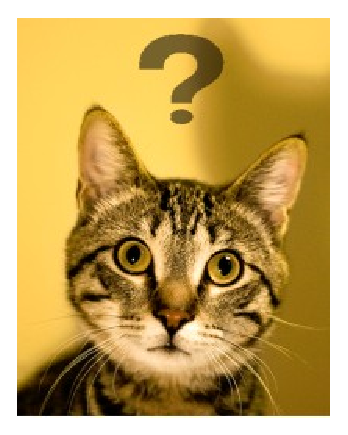
\includegraphics[scale=0.5]{images/confused_cat.eps}
    \end{wrapfigure}

  Characteristics:
    \begin{itemize}
      \item created and published by Guido Van Rossum in 1991
      \item Interpreted
      \item Multiplatform
      \item Object Oriented
      \item Dynamic Typing
      \item Coding Style
    \end{itemize}

  \end{frame}

  \begin{frame}{How to Start Python?}
    
    You can either run python from a script or Interactively:

    \begin{block}{Interactive:}
      \scriptsize
      (using the interpreter to run python code)\\
      \textdollar \ python\\
      \textgreater\textgreater\textgreater \ print "Hello there!"\\
      Hello there
    \end{block} 

    \begin{block}{From a script:}
      \scriptsize
      (using a text file with python code)\\
      \textdollar \ python myscript.py\\
      Hello there!\\
      \textdollar
    \end{block}

  \end{frame} 

  \begin{frame}{Data types in Python}

    {\bf Numbers:} Integer(42), float(13.37), complex(12+3n)\\
    {\bf Strings:} "nothing interesting here move along"\\
    {\bf Dictionaries:} dict = \textbraceleft name : `Maria', age : 22, 42 : `haha' \textbraceright \\
    {\bf Lists:} list = [1, `classic', 2, `boring']\\
    {\bf Tuples:} tuple = ( 1, 2, 42, `Maria', (1,2,3) )\\
    {\bf Objects:} instance = Class(`foobar')\\
    {\bf Modules:} import antigravity

  \end{frame}

  \begin{frame}{Python has objects!}
    
    Everything in python is an object and every object has its attributes.

    \begin{block}{Object Attributes:}
      \scriptsize
      \textgreater\textgreater\textgreater \ name = `maria'
      
      \textgreater\textgreater\textgreater \ name.index(`i')\\
        3
      
      breaking down the above statement we have:
        \begin{itemize}
          \item variable
          \item delimeter
          \item attribute
          \item parameters (if any)
        \end{itemize}
    \end{block}

  \end{frame}

  \begin{frame}{Another peek in Attributes/Methods}

    \begin{figure}
      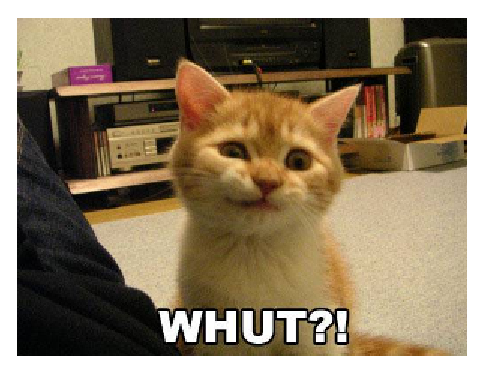
\includegraphics[scale=0.5]{images/whut.eps}
    \end{figure}

    Attributes?! Methods?! i can't remember all these stuff!

    \begin{block}{Lucky you! you dont have to know all of them}
      \scriptsize
      using dir():
      dir allows you to peek into an object and learn about its supported methods\\
      lets take a look at a list for example.
      \textgreater\textgreater\textgreater \ dir(list):\\ \
      [`append', `extend', `insert', `remove', `pop', `index', `count', `sort', `reverse']
    \end{block}
  
  \end{frame}

  \begin{frame}{Back to data type fun}{Dictionaries}

    \begin{block}{Example}
      \scriptsize
      \textgreater\textgreater\textgreater \  dict = \textbraceleft name : `Maria', age : 22, 42 : `haha' \textbraceright \\
      
      \textgreater\textgreater\textgreater \ dict['age']\\
        22\\
      \textgreater\textgreater\textgreater \ `name' in dict\\
        True\\
      \textgreater\textgreater\textgreater \ del dict['age']\\
      (we could also use pop to also return the removed key's value)
    \end{block}
    
  \end{frame}

  \begin{frame}{Back to data type fun}{Lists}

    \begin{block}{Example}
      \scriptsize
      \textgreater\textgreater\textgreater \ list = [1, `classic', 2, `boring']\\

      \textgreater\textgreater\textgreater \ list.append("Maria")\\
      \textgreater\textgreater\textgreater \ list

        [1, `classic', 2 `boring', `Maria']\\
      \textgreater\textgreater\textgreater \ list.insert(4,"Alex")\\

      \textgreater\textgreater\textgreater \ list

        [1, `classic', 2 `boring', `Alex', `Maria']
    \end{block}
    
  \end{frame}

  \begin{frame}{Back to data type fun}{Tuples}

    Tuples also known as Sequences and as such they are {\bf ordered}.
    you can also slice them using the {\bf slice operator:}

    \begin{block}{Slice Operator}
      \scriptsize
      mysequence[ i : j ]
      
      with `i' and `j' being your range in the sequence ( i = start , j = one past the end )
    \end{block}

    \begin{block}{Example}
      \scriptsize
      tuple = ( 1, 2, 42, `Maria', (1,2,3) )\\

      \textgreater\textgreater\textgreater \ tuple[0]\\
        1\\
      \textgreater\textgreater\textgreater \ tuple[3]\\
        `Maria'\\
      \textgreater\textgreater\textgreater \ tuple[1:2]\\
        (1,42)\\
      \textgreater\textgreater\textgreater \ tuple[-1]\\
        (1,2,3)\\
      \textgreater\textgreater\textgreater \ tuple[3:]\\
        (`Maria',(1,2,3))
    \end{block}

  \end{frame}
  
  \begin{frame}{Python type mutability}
    
    The value of some objects can change. Objects whose value can change are said to be mutable;\\
    objects whose value is unchangeable once they are created are called immutable.
    \begin{block}{mutable}
      Dictionaries, Lists
     \end{block}
     \begin{block}{immutable}
       Numbers, Strings, Tuples, Frozensets
     \end{block}

  \end{frame}

  \begin{frame}{Flow Control}{Conditionals}

    \begin{block}{IF statement}
    name = "Maria"

    if name == "Maria":\\
    \ \ \ \ print "Hello Maria!"\\
    elif name == "George":\\
    \ \ \ \ print "Hello George!"\\
    else:\\
    \ \ \ \ print "Hello stranger!"\\
    \end{block}
    
  \end{frame}

  \begin{frame}{Flow Control}{Loops}
    
    \begin{block}{While loop}
      i = 0\\
      while i\textless5:\\
      \ \ \ \ print i\\
      \ \ \ \ i += 1\\
    \end{block}

  \end{frame}

  \begin{frame}{Flow Control}{Loops}

    \begin{block}{for loop}
      for item in range(1,100):\\
      \ \ \ \ print item\\
    \end{block}
    \begin{block}{yet another for loop}
        names = ("Maria", "George", "Helen", "Alex")\\
        
        for item in names:\\
        \ \ \ \ print item\\
    \end{block}
    
  \end{frame}

  \begin{frame}{Numeric Operators}
    
    {\bf + - * /} \ \ \ Your everyday numeric operations.\\
    {\bf \%} \ \ \ Modulus - Divides left hand operant by right hand operant. 
      
    \ \ \ \ \ \ \ Returns `Remainder'\\
    {\bf **} \ \ \ Exponent - performs exponential calculation on operant.\\
    {\bf //} \ \ \ Floor Division - division operant where the digits after the 
    
    \ \ \ \ \ \ \ result's decimal point are removed.

  \end{frame}

  \begin{frame}{Function Definition}
     
    \begin{block}{a simple function}
      \scriptsize
      \textgreater\textgreater\textgreater \ def foo(bar):\\
      \ \ \ \ \ \ \ \ \ \ \ \ \ print bar\\
      \textgreater\textgreater\textgreater \ foo(123)\\
      \ \ \ \ 123
    \end{block}

  \end{frame}
  
  \begin{frame}{Class Definition}
    
    \begin{block}{a simple class}
      \scriptsize
      class AddressBookEntry(object):\\
      \ \ \ \ def \_\_init\_\_(self, name, phone):\\
      \ \ \ \ \ \ \ \ self.name = name\\
      \ \ \ \ \ \ \ \ self.phone = phone\\

      \ \ \ \ def update\_phone(self, phone):\\
      \ \ \ \ \ \ \ \ self.phone = phone\\
    \end{block}

  \end{frame}
\end{document}
